\section*{Section4.1}

\begin{enumerate}
    %\item 对低马赫数均熵流动绕过静止物体的声辐射问题, 
    %假设声源区域声学紧致, 观察点 \(\boldsymbol{x}\) 位于声学远场。
    %假设近场区域流动信息已知, 且勿略黏性影响, 
    %从涡声方程出发, 证明观察点 \(x\) 的声场可表示为
    %\[  
    %p^{\prime}(\mathbf{x}, t)=\int_{S} p^{\prime}(\mathbf{y}, \tau) \frac{\partial G}{\partial y_{i}} n_{i} \mathrm{dS}(\mathbf{y}) \mathrm{d} \tau-\rho_{0} \int(\boldsymbol{\omega} \times \mathbf{u})_{i}(\mathbf{y}, \tau) \frac{\partial G}{\partial y_{i}} \mathrm{~d}^{3} \mathbf{y} \mathrm{d} \tau
    %\]
    \item 考虑平面波在非均匀流中的传播, 
    假设声速整场均匀, 平均流速度沿水平方向 且与纵坐标轴呈线性关系。
    绘图分析平面波向上游传播时路径的变化趋势。
        \vspace{-0.5cm}
        \begin{figure}[htbp]
            \centering
            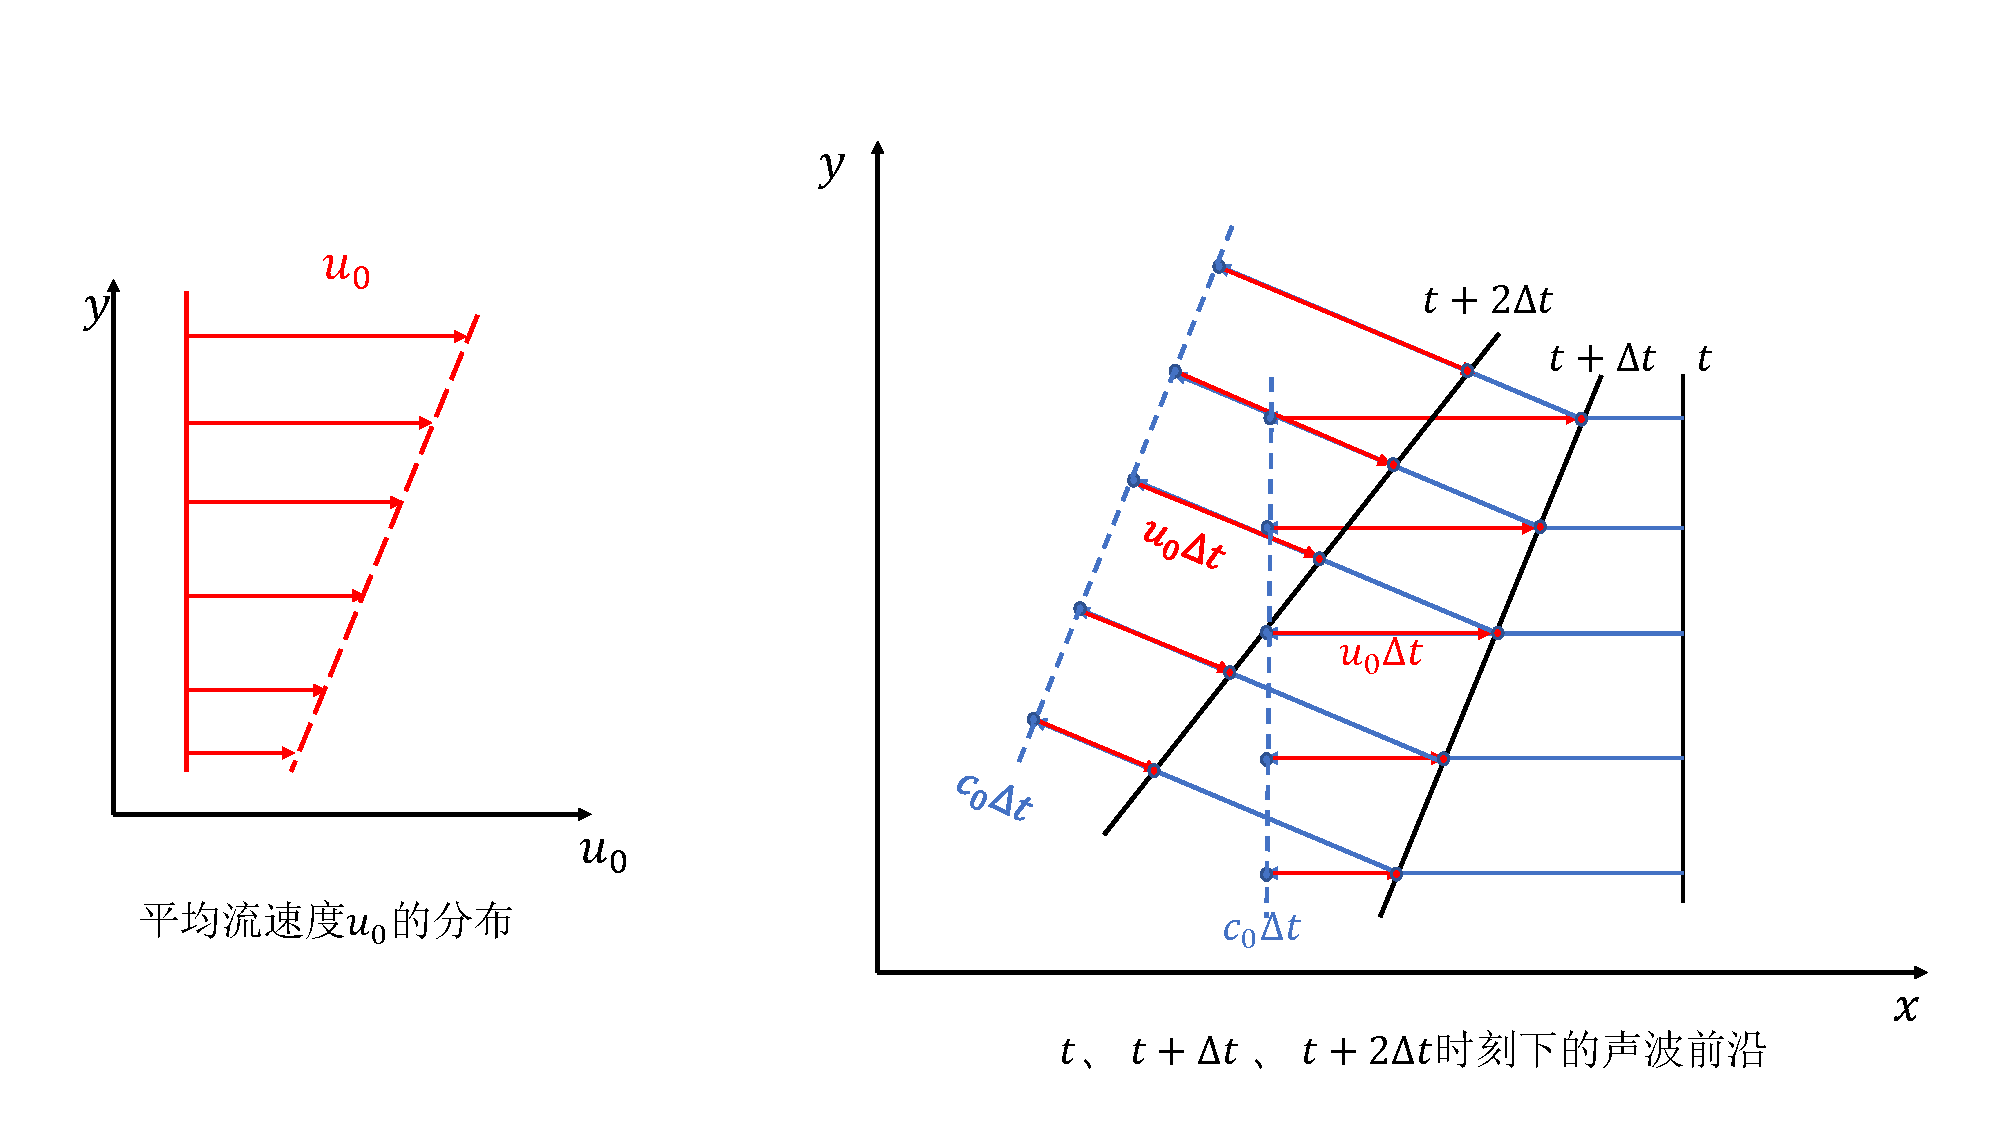
\includegraphics[height=8cm]{image/Section4.1_1.pdf}
        \end{figure}
        
        平面波向上游传播时路径的变化如右图所示。
        当平均流速度\(u_{0}\)分布如左图所示时,
        平面波向上游传播会朝着纵坐标轴的正方向偏转,
        即向着速度较大的方向偏转。

    \item 声衬的消声作用跟边界层厚度与波长的比值有关,
    比值越小消声作用越弱, 试分析原因。
        
    由于流体在边界层的速度梯度,
    声波在传播时会朝着声衬方向偏转,
    当边界层厚度与波长的比值变小时,
    边界层对声波的偏转作用变弱,
    传播到声衬的声波变少,
    消声作用减弱。

\end{enumerate}

\clearpage